
Modern service robots are designed to understand human instructions and complete tasks in real-world household environments (e.g., ``Turn off the TV if it is currently on," ``Bring the red pillow from the living room to the bedroom"). This process involves interpreting natural language commands, generating and answering relevant questions for scene understanding and reasoning (e.g., ``Is the TV turned on?" ``What is the color of the pillow?"), and manipulating target objects accordingly. 
A crucial step is answering these questions, a task known as Embodied Question Answering (EQA)~\cite{das2018embodied}, which requires robots to efficiently explore the 3D environment from a random starting location and actively gather information until a confident answer can be provided. 
Prior studies have investigated this in single-agent settings \cite{das2018embodied,ren2024explore,majumdar2024openeqa,yu2019multi,yao2025towards}. In contrast, we envision future households with multiple \textit{heterogeneous} service robots, each with distinct capabilities and non-transferable assignments. While they cannot take over each other's tasks, they can access all generated questions and share observations and interpretations to enhance exploration efficiency. We define this cooperative information-gathering setting as a \emph{multi-agent multi-task EQA (MM-EQA)} problem, a novel challenge that facilitates multi-robot collaboration in real-world scenarios.

\begin{figure}[!tbp]
    \centering
    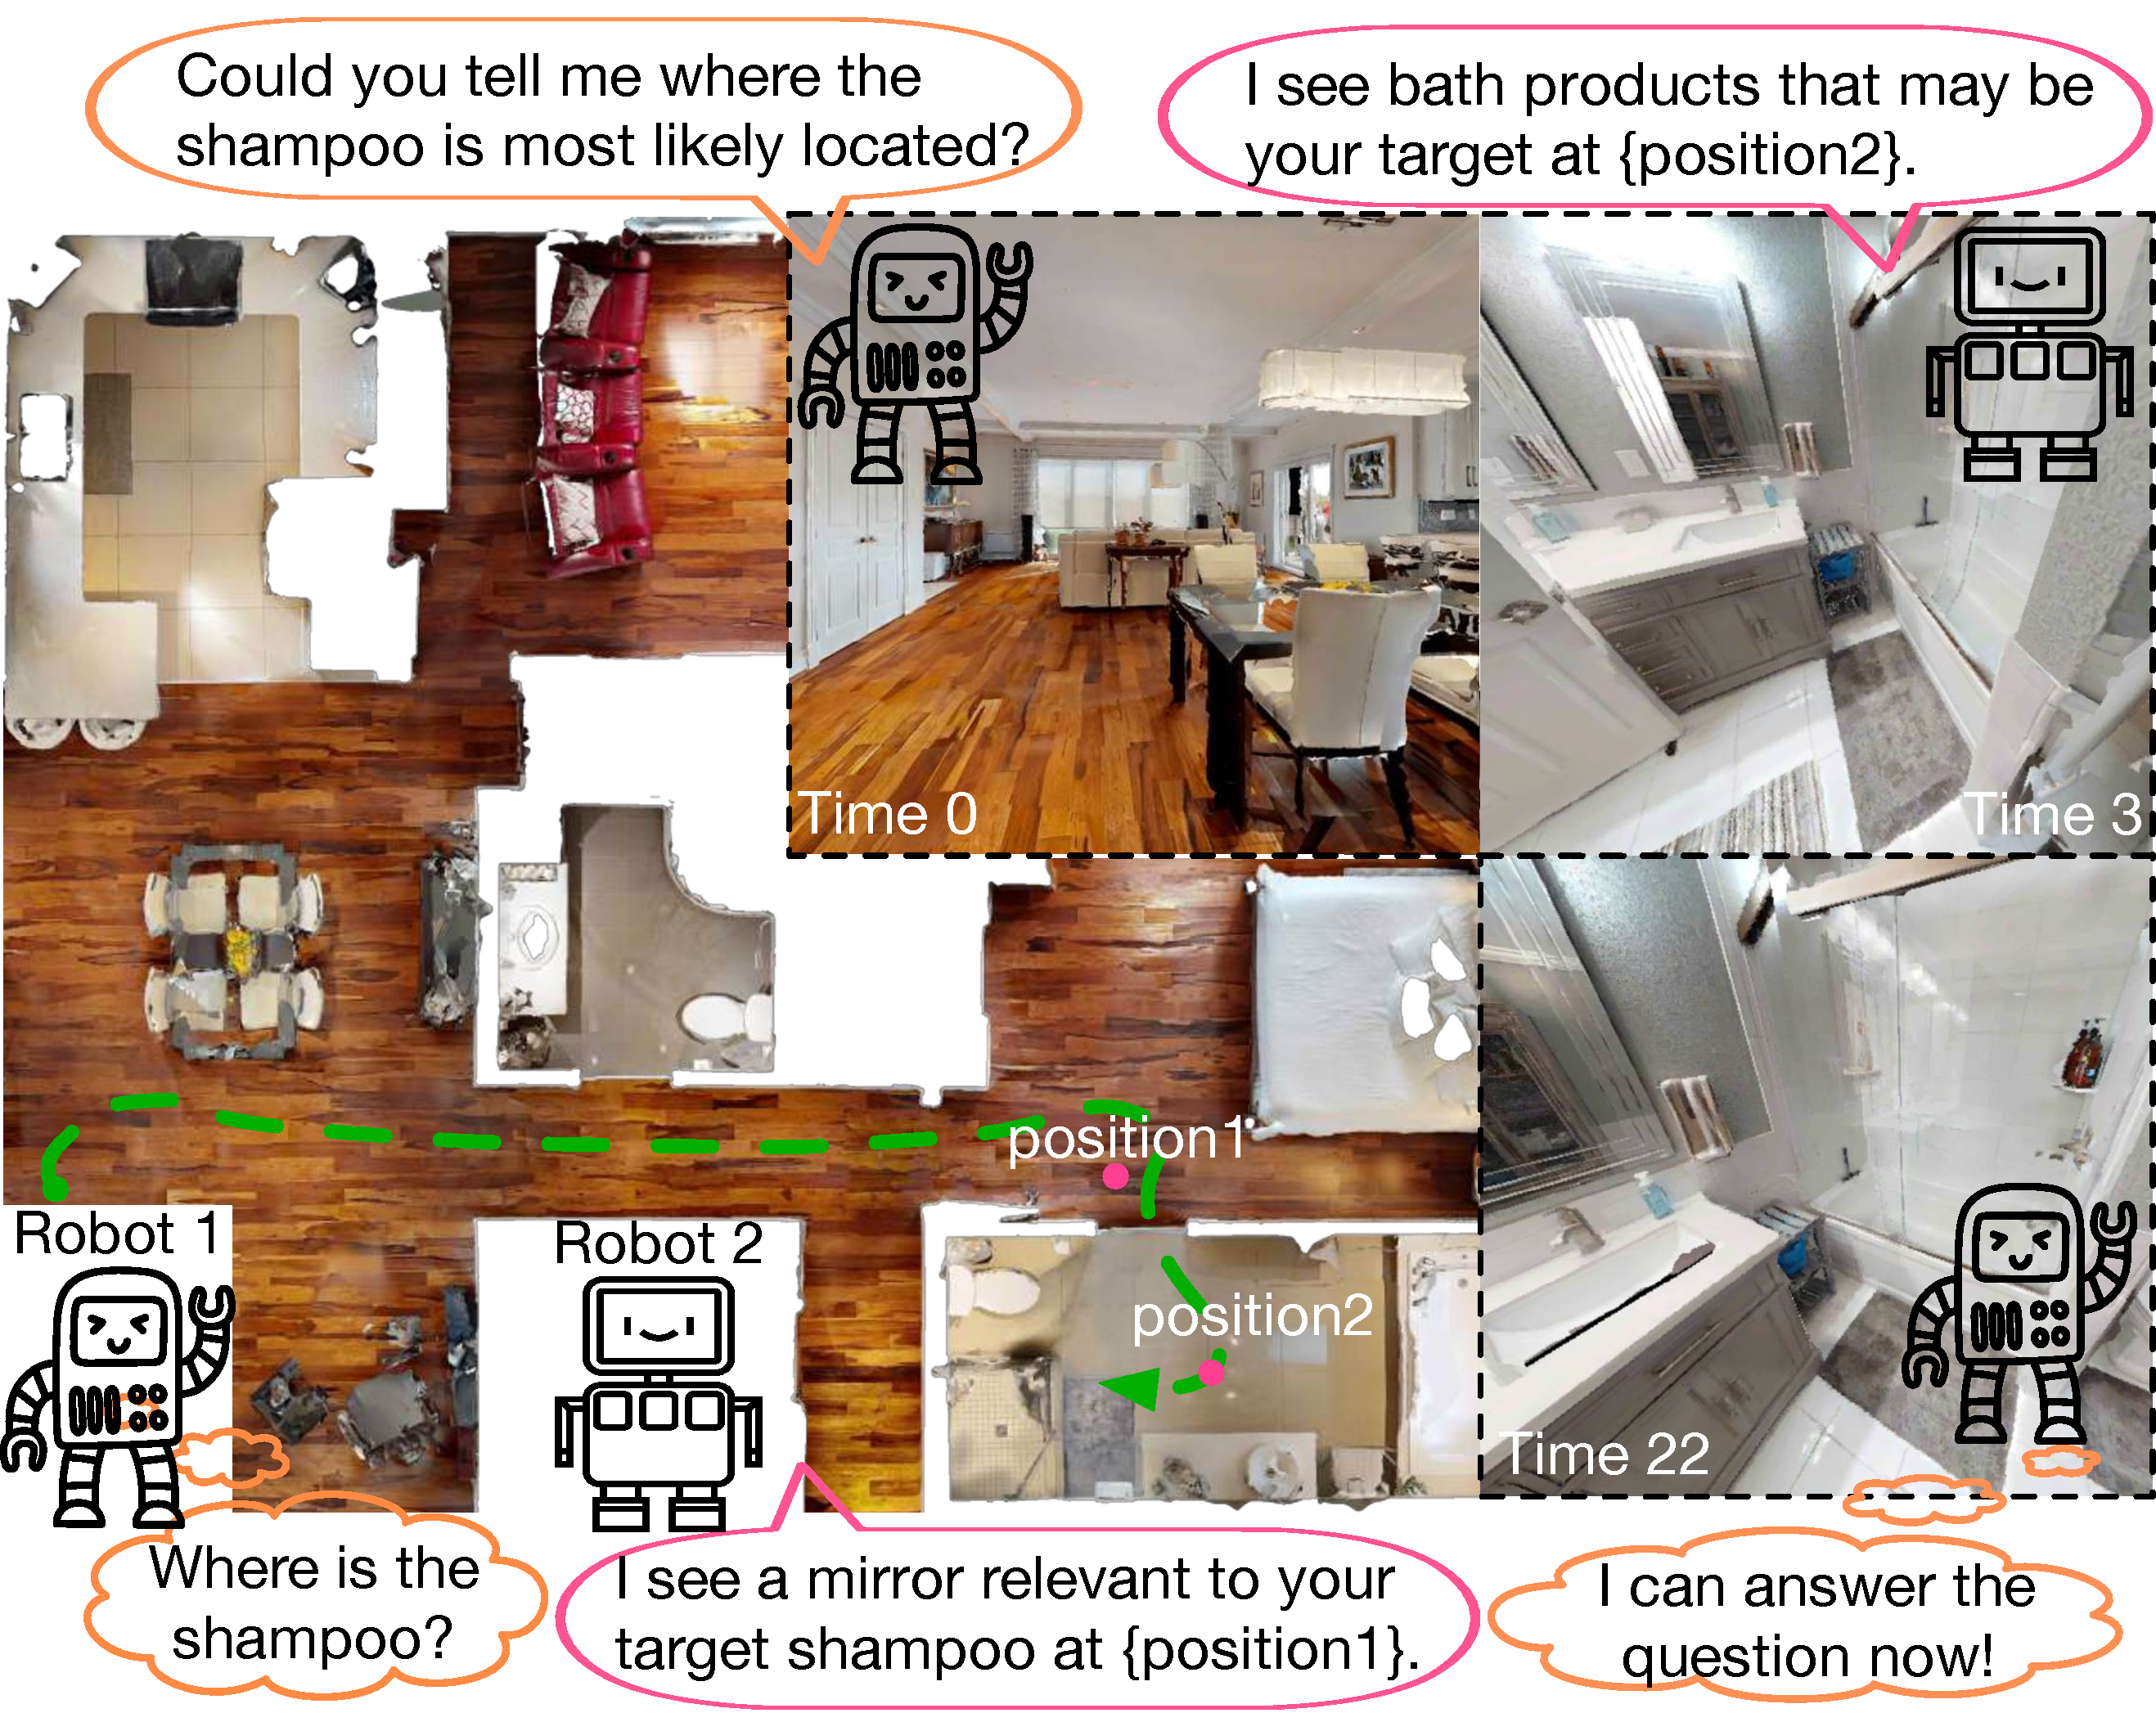
\includegraphics[width=1\linewidth]{img/Fig.pdf}
    \vspace{-0.7cm}
    \caption{In a household setting, robots exchange observations and reasoning to collaboratively complete their assigned tasks. Each agent generates confident and goal-directed messages using calibrated outputs from LLMs. The bottom-left image shows a bird’s-eye view of Robot 1’s navigation path after incorporating information received from Robot 2. The top-right sequence captures both robots’ camera views at different timestamps.}
    \vspace{-0.7cm}
    \label{fig:intro}
\end{figure}


While existing single-agent EQA solutions can be adapted to a multi-agent setting by having each robot work independently, this naive approach is inefficient. 
Communication enables mutual assistance, improving exploration and increasing the likelihood of faster task completion. 
However, uncalibrated communication could hinder efficiency by sharing irrelevant or misleading information. 
Therefore, it is critical to ensure that messages are accurate and pertinent to the recipient's tasks.
This work tackles the MM-EQA problem by designing a communication framework that enhances multi-agent exploration efficiency and task performance.

Large language Models (LLMs) have shown great potential in solving EQA tasks due to their remarkable ability to understand natural-language queries, reason, and provide answers in natural language~\cite{zhang2023building}. 
In the context of MM-EQA, natural language is an ideal communication protocol, as LLMs are inherently trained to engage in dialogues. Several LLM-based communication methods have been proposed in other domains~\cite{zhang2024towards,rasal2024llm}, but these cannot be directly adapted to our MM-EQA setting. 
Additionally, LLMs often produce miscalibrated and overconfident outputs~\cite{ mielke2022reducingconversationalagentsoverconfidence}, which can result in irrelevant or misleading information. 
This can hinder cooperation efficiency, as agents may share inaccurate data, reducing overall exploration effectiveness~\cite{hao2024quantifying}.

Our work tackles this challenge and develops an LLM-based communication framework for MM-EQA. Our key insight is that \emph{an agent should only communicate information it confidently deems relevant to its partner agents' tasks} (see Fig. \ref{fig:intro}).
We propose CommCP, a novel decentralized LLM-based communication framework that employs conformal prediction (CP) \cite{shafer2008tutorial,ren2023robots} to calibrate the confidence of LLM's outputs. 
Our framework ensures that the outputs generated by LLMs are more reliable and reduces the negative impact of irrelevant or misleading information to partner agents, ultimately enhancing the overall task performance and efficiency of the multi-agent system.
To evaluate our proposed framework, we create a novel MM-EQA benchmark based on realistic scenarios and the Habitat-Matterport 3D (HM3D) dataset \cite{ramakrishnan2021habitat}.
The experimental results show that our approach enhances the task success rate and shortens completion time by a large margin over baselines.

The main contributions of this paper are as follows:
\begin{itemize}
    \item We formulate the information-gathering process of completing assignments provided in natural language as a novel multi-agent multi-task embodied question answering (MM-EQA) problem, where multiple robots work as a team, handling EQA tasks in a shared environment and communicating to exchange information or answers.
    \item We propose CommCP, a novel LLM-based decentralized communication framework for MM-EQA, where conformal prediction is employed to calibrate the generated messages to reduce distractions to other agents and improve communication reliability and efficiency. 
    \item We create a novel MM-EQA benchmark with photo-realistic scenarios from the HM3D dataset to validate the effectiveness of the proposed framework. This benchmark is released to facilitate future studies.
\end{itemize}